\chapter{Rocketry}
\index{rockets}

Rockets propel hot gases, which recreates an equal and opposite reaction that pushes it forwards, even in a vacuum. 

Even without anything to push against, the rocket can still move forward thanks to Newton's Third Law. 

Imagine a spacecraft with a bowling ball attached to the back. If that spacecraft exerts a force to throw the bowling ball backwards, the ball will exert a force on the ship, moving it forwards. 

\begin{figure}[htbp]
    \centering
	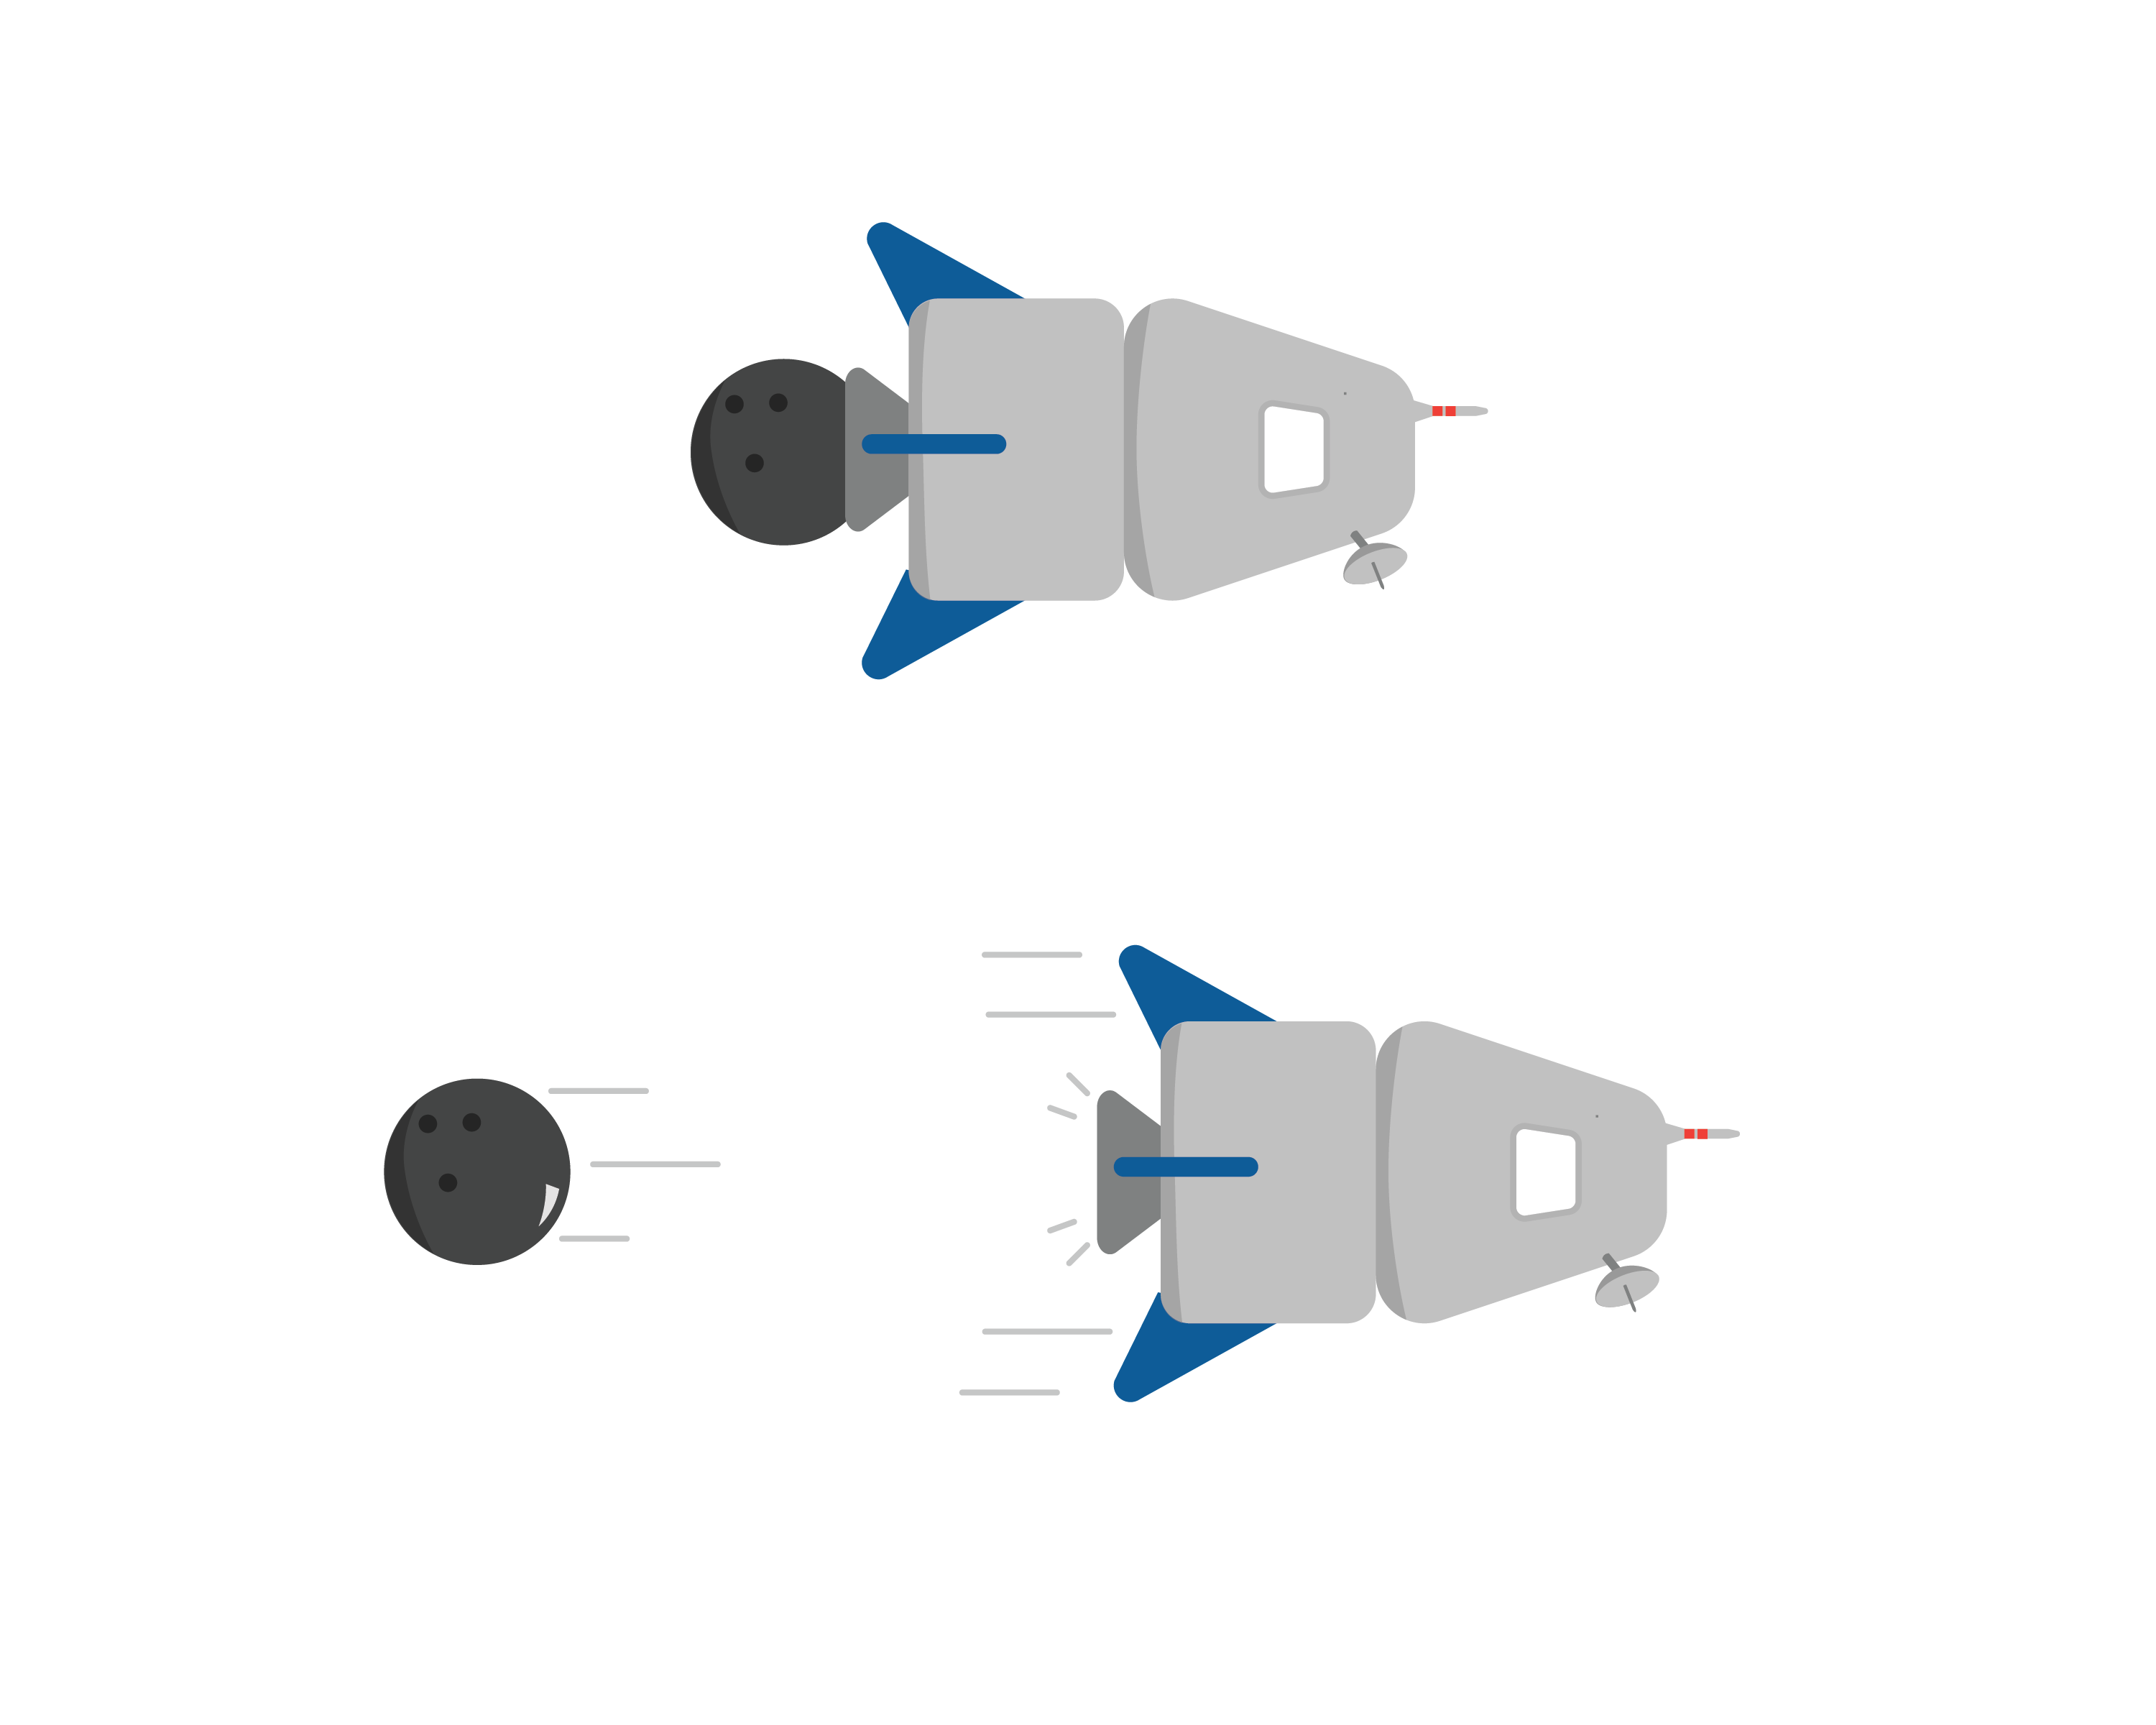
\includegraphics[width=0.75\textwidth]{thirdLaw.png}
    \caption{Newton's Third Law in action .}
    \label{fig:example}
\end{figure}


Instead of a bowling ball, real-life rockets usually "throw" particles of hot gas at very high speeds. Rockets carry their own oxidizer to provide oxygen to allow fuel to burn. 

\section{Types of rocket fuels}

There are two main types of chemical rockets. 

One type is a \newterm{Solid Fuel Rocket}, which ignites a solid fuel-oxidizer mix. Once the solid fuel is ignited, it can't be stopped until all of the fuel is exhausted.

\begin{figure}[htbp]
    \centering
	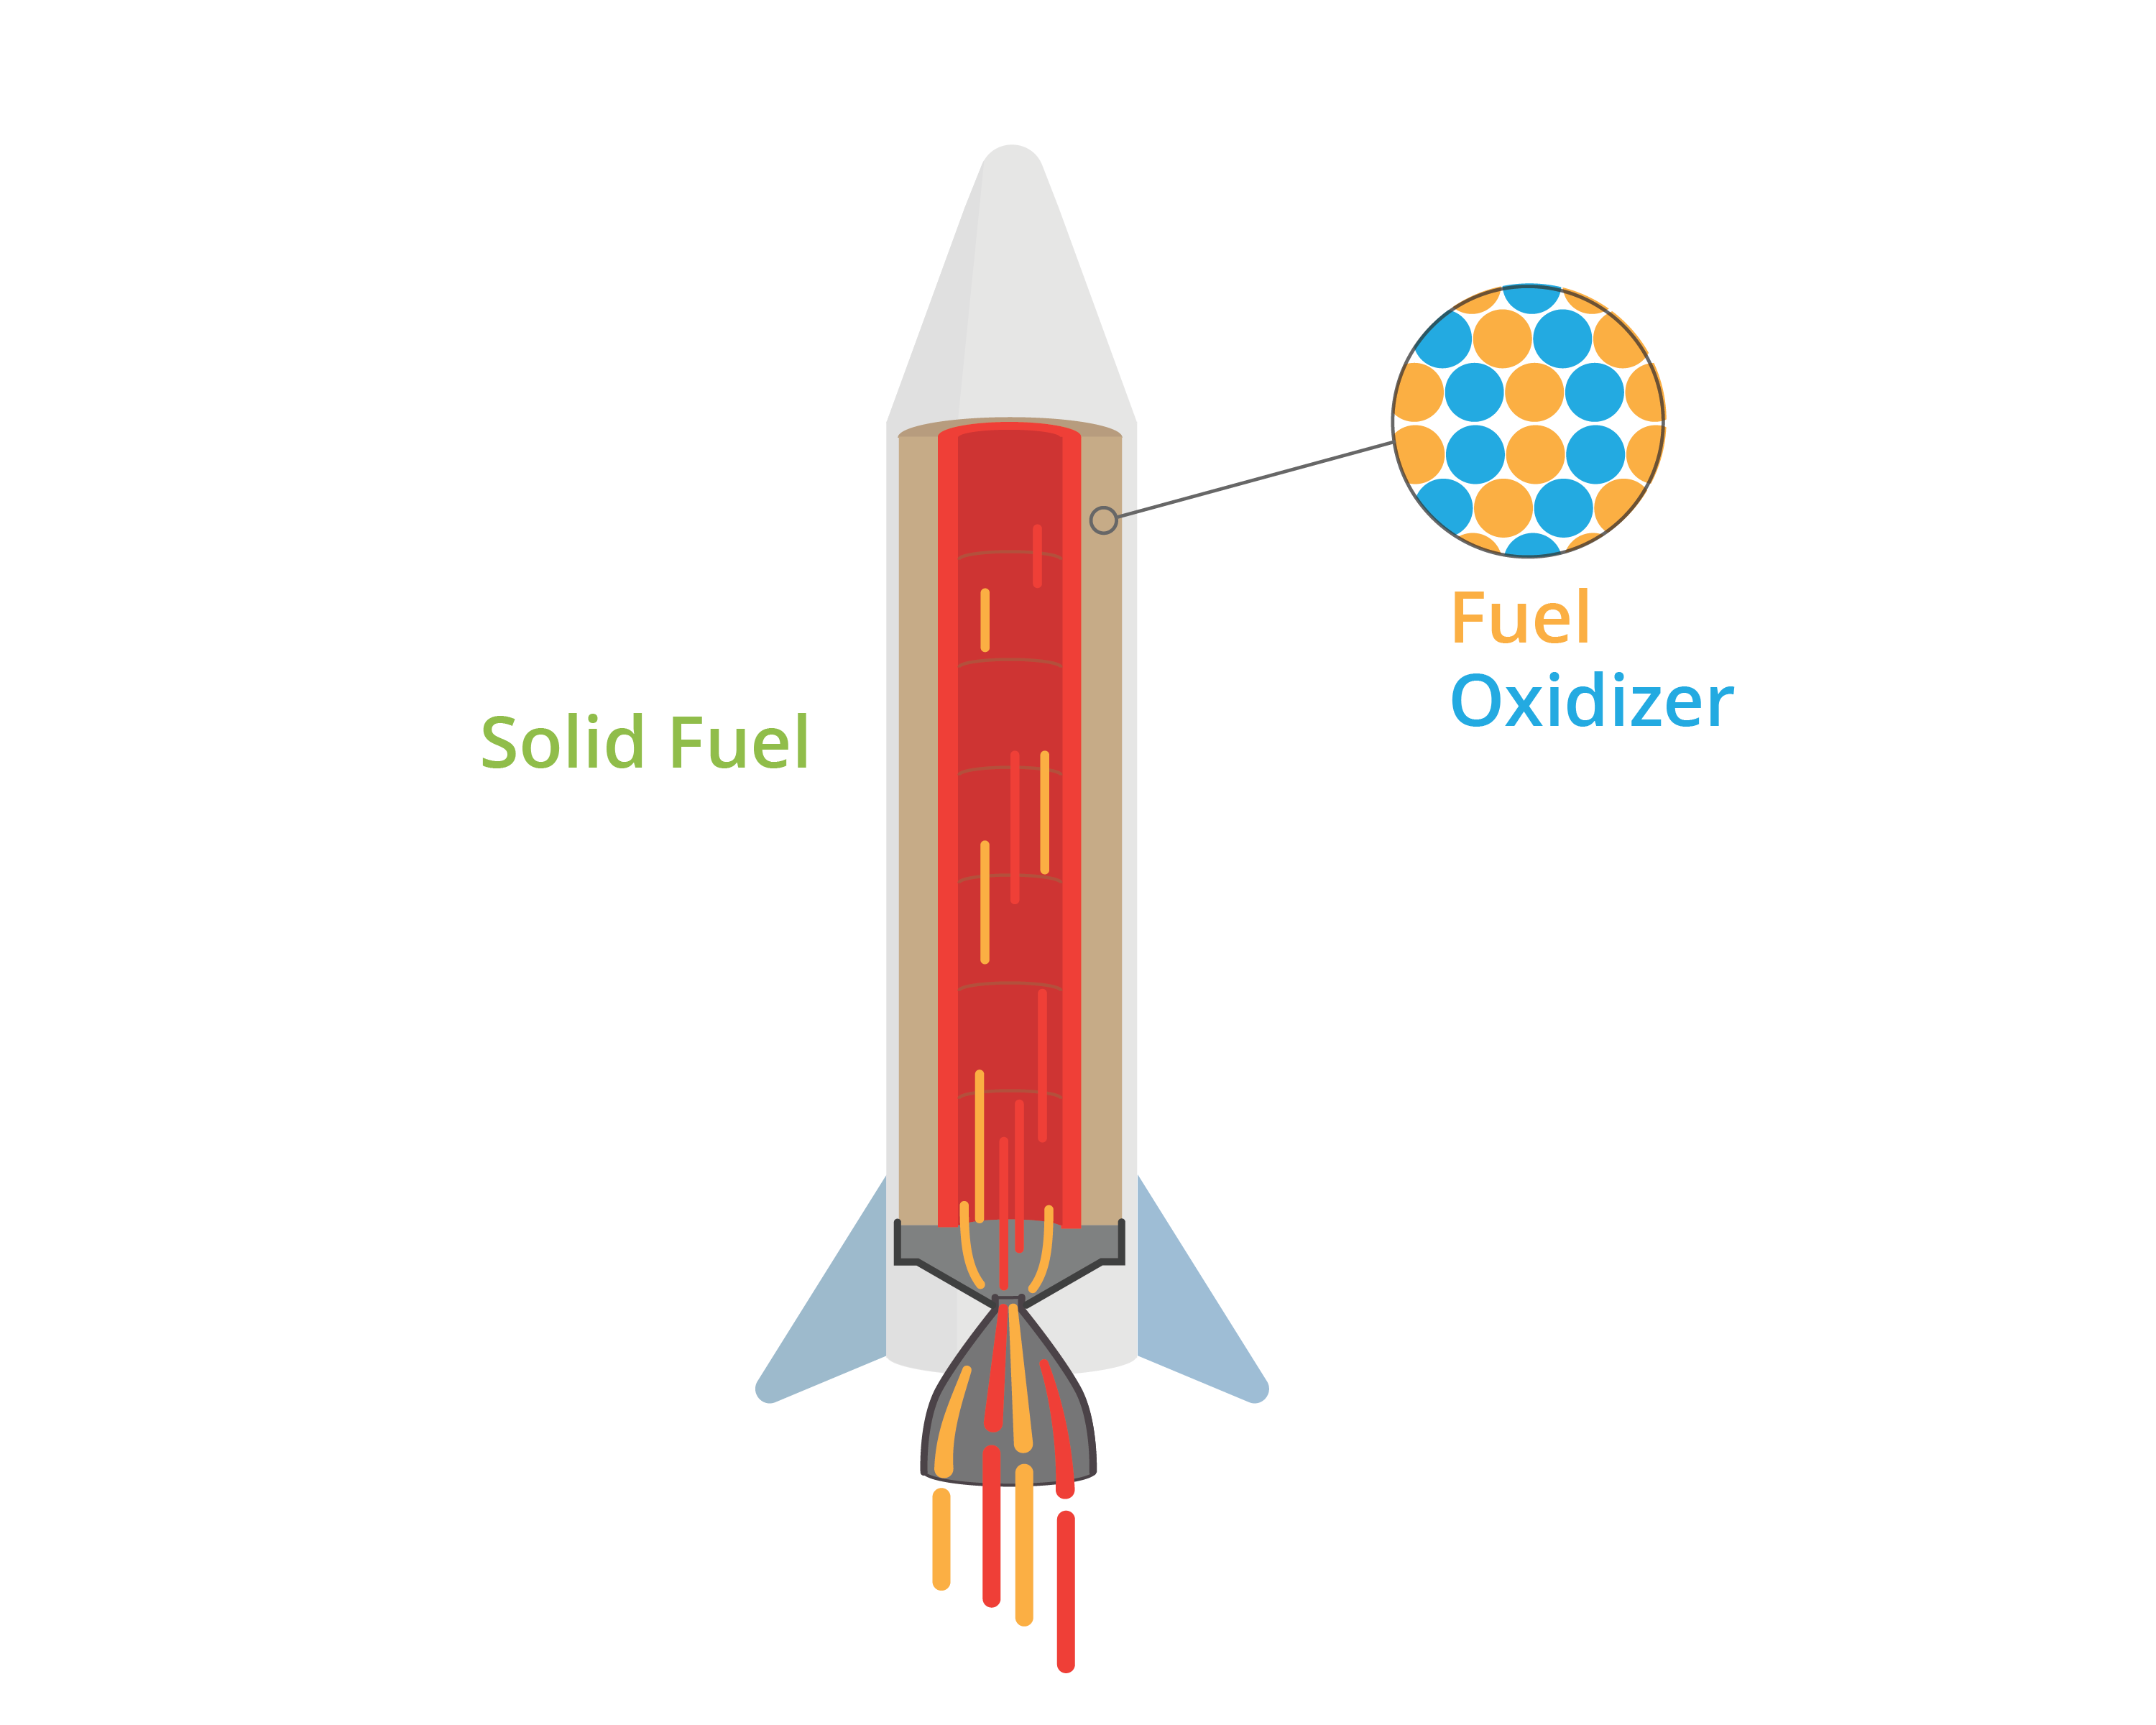
\includegraphics[width=0.75\textwidth]{solid.png}
    \caption{A solid fuel-oxidizer rocket.}
    \label{fig:solidfuel}
\end{figure}

The other main type of chemical rocket is called a \newterm{Liquid Fuel Rocket}. Liquid fuel rockets contain separate tanks for liquid fuel and liquid oxygen. Fuel pumps bring them both to a combustion chamber where they ignite and exit the rocket. Most liquid fuel engines can control their thrust. 
\index{rockets ! liquid fuel based}

\begin{figure}[htbp]
    \centering
	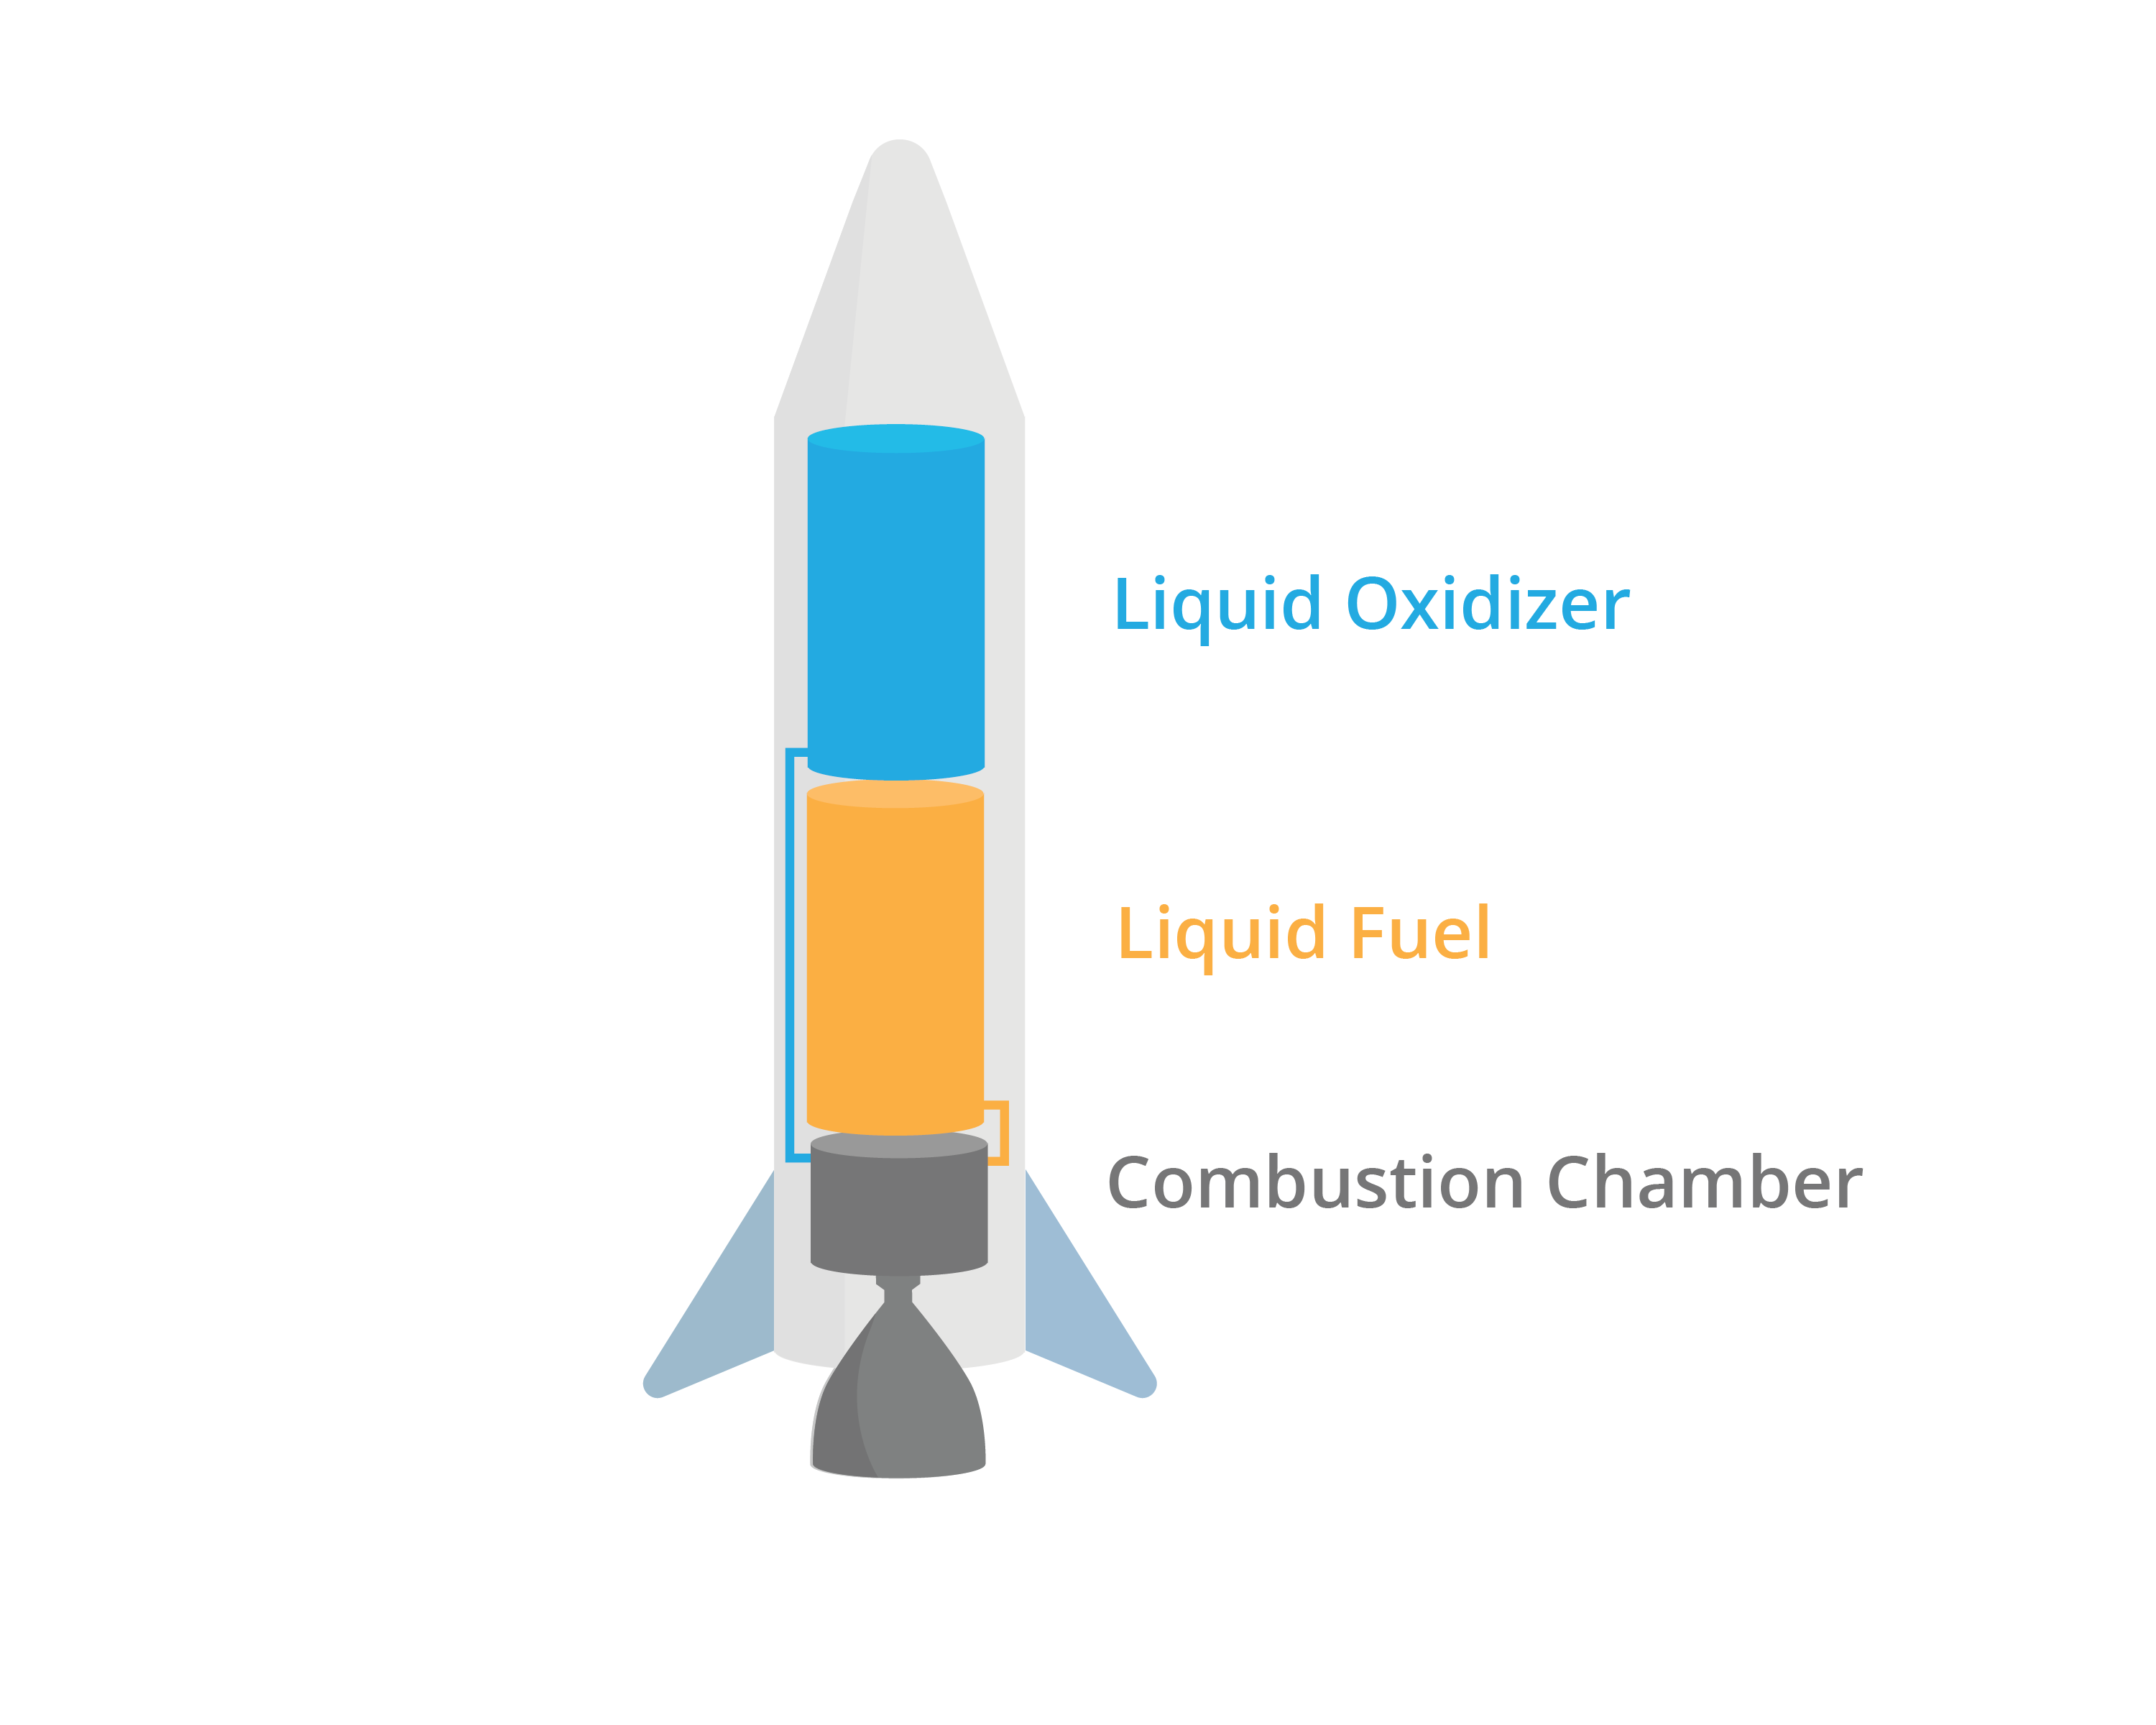
\includegraphics[width=1\textwidth]{liquid.png}
    \caption{A liquid chemical phase.}
    \label{fig:liquidfuel}
\end{figure}


\section{Tyranny of the rocket equation}
	Chemical rockets can only burn the fuel that they bring with them. However, the more fuel you carry, the heavier the vehicle will be.

 

	One way to help reduce this weight is by using \newterm{staging}. 
	\index{rockets ! staging}
	\begin{figure}[htbp]
    \centering
	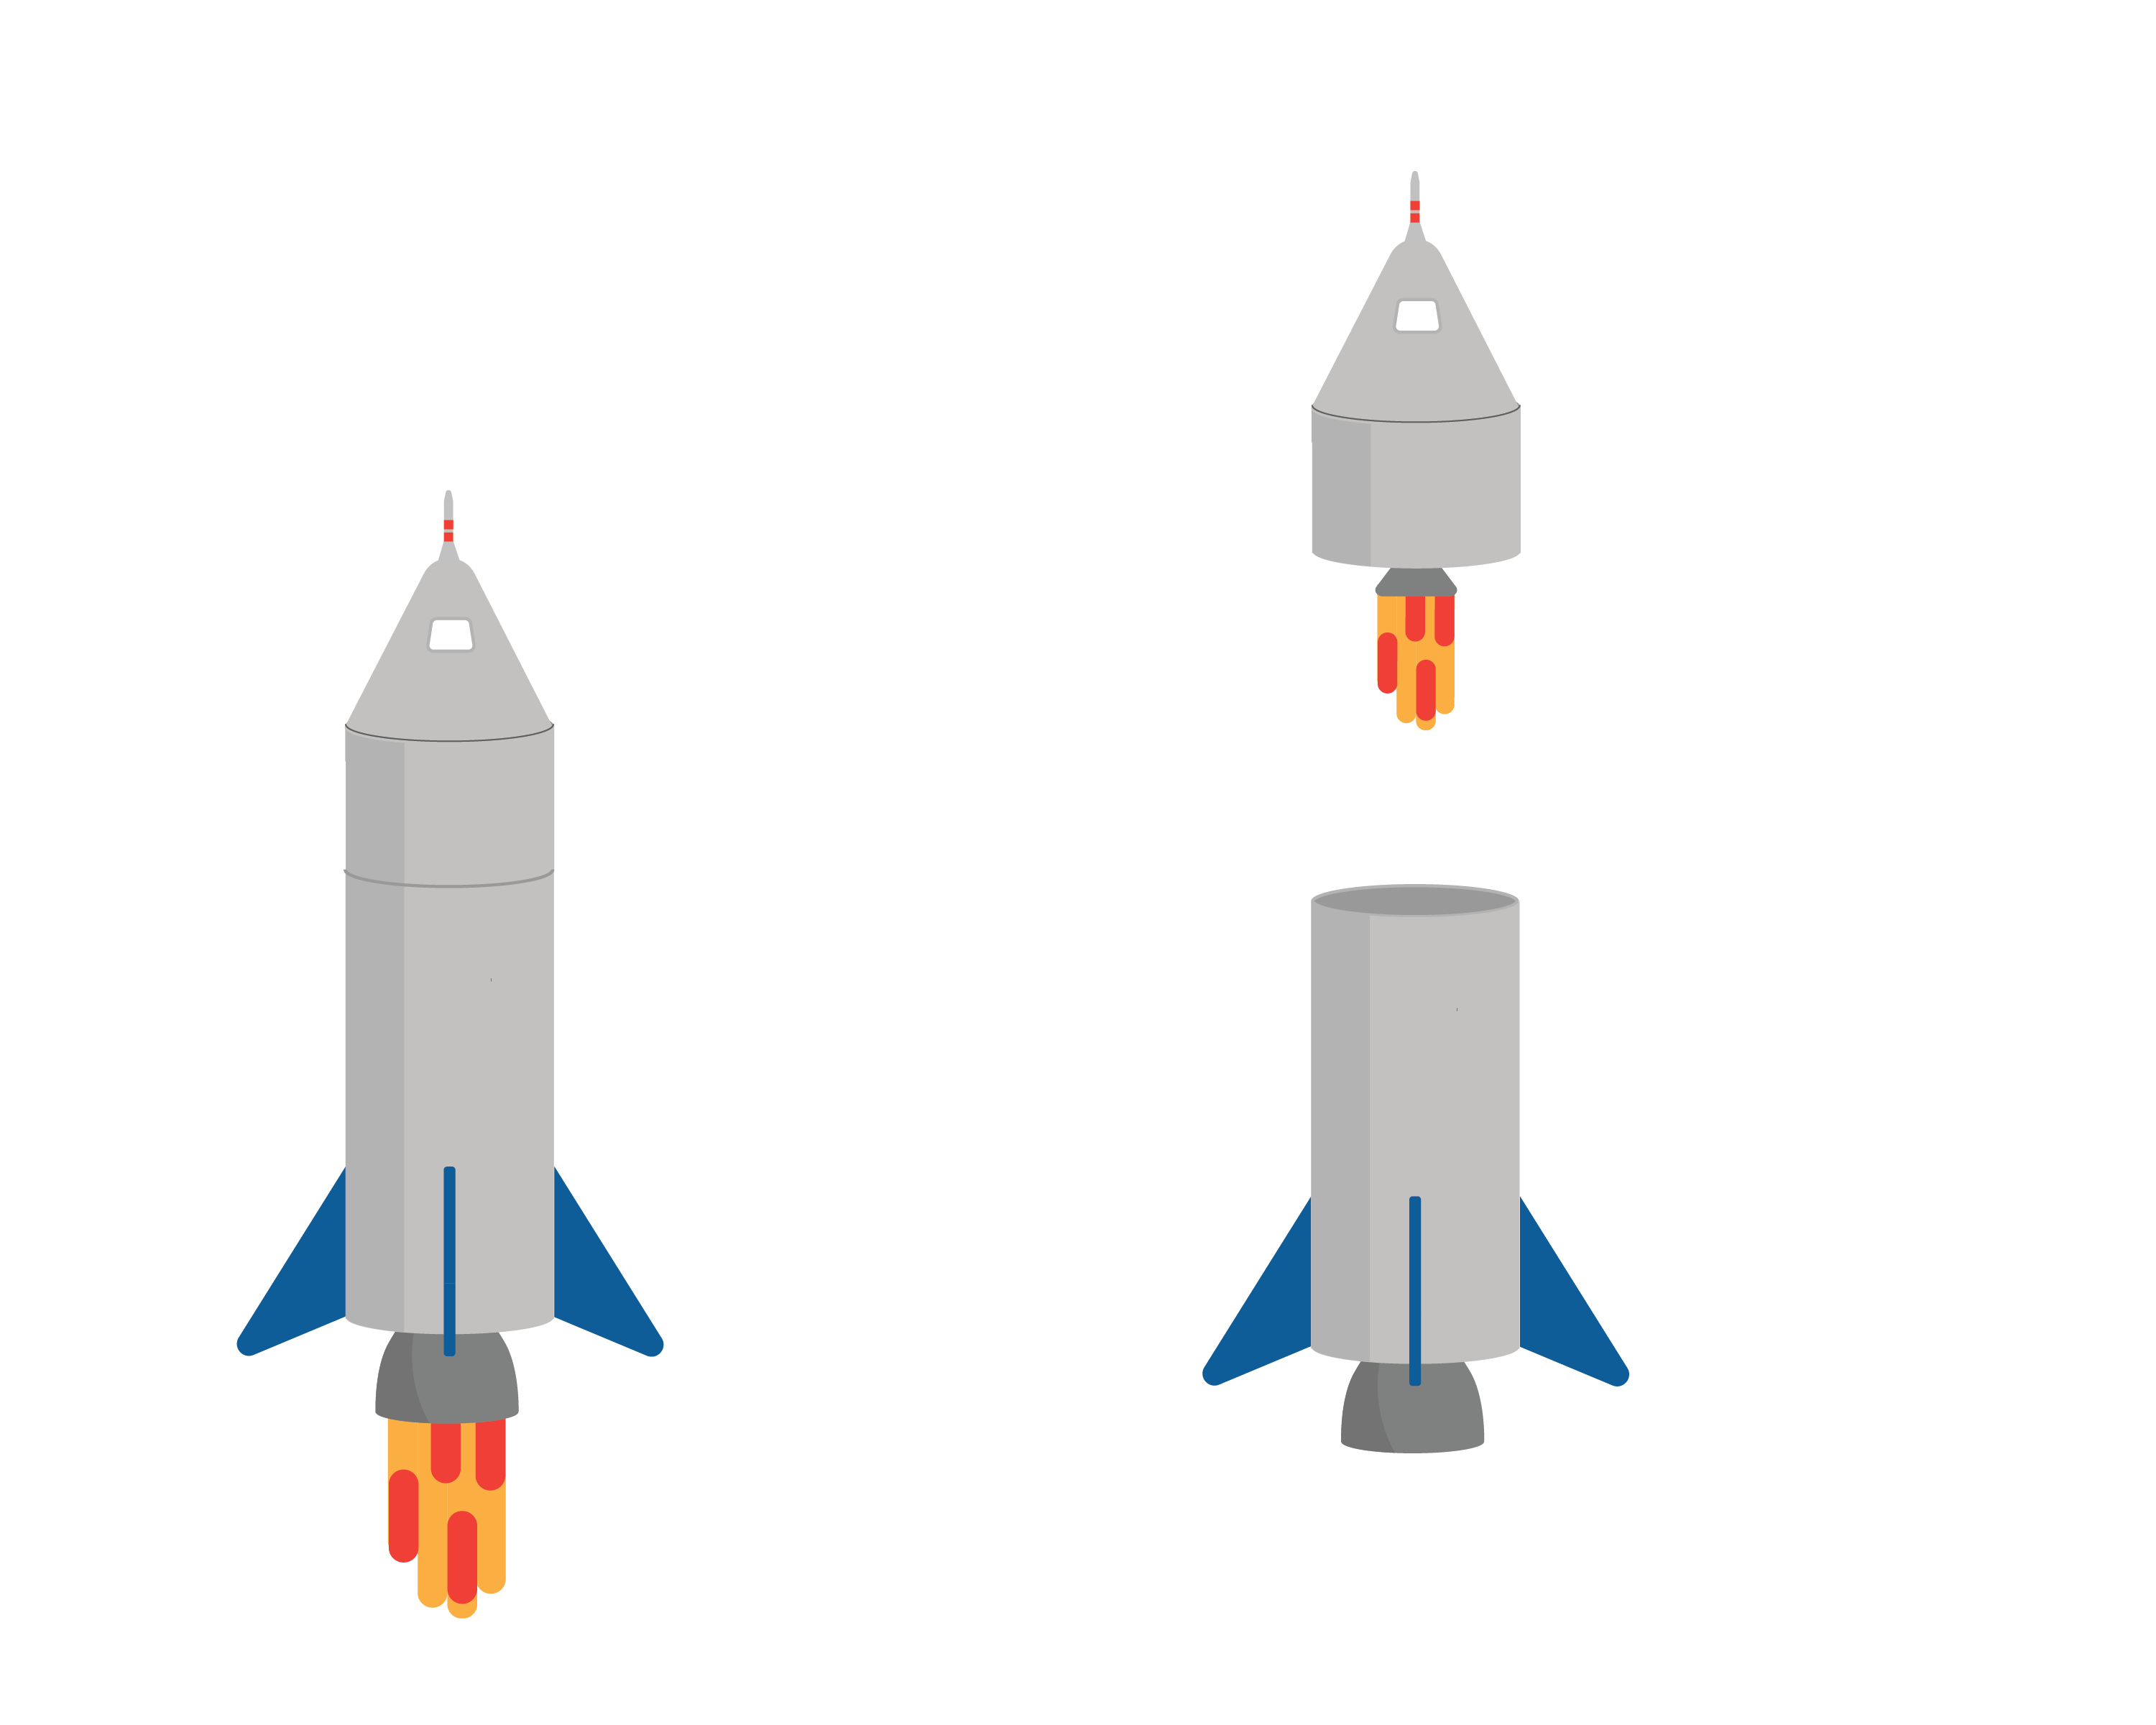
\includegraphics[width=0.75\textwidth]{stagingDual.png}
    \caption{A dual stage rocket eliminates one of its stages throughout flight.}
    \label{fig:dualStaged}
\end{figure}
	Staging allows rockets to drop unnecessary structural mass once they've used up a certain amount of fuel. 



\section{Control in atmosphere} 
\index{rockets ! in atmosphere}
There are several common ways that engineers have managed to control rockets' direction in the atmosphere. Usually, on-board sensors detect the orientation of the rocket, and can automatically adjust these controls to keep the rocket going the correct direction.

	
	One method is using \newterm{movable fins}. The fins work similarly to control surfaces that we covered in the airplanes chapter. 

	Another method of control uses a \newterm{gimbaled engine}. A gimbaled engine is an engine that can pivot in a certain direction. 
	By pivoting the engine, the rocket can change its direction of thrust, which changes the direction of the rocket. This is called \newterm{thrust vectoring}. 

	A more outdated method is using \newterm{vernier engines}, which are two smaller engines that control attitude. However, this adds a large amount of weight to the rocket, so they are less frequently used today.

	\subsection*{Pros and Cons of Rocket Control Systems in Atmosphere}

	\begin{itemize}
		\item \textbf{Movable fins}
		\begin{itemize}
			\item \textbf{Pros:} Simple, reliable, lightweight, effective at high speeds in atmosphere.
			\item \textbf{Cons:} Ineffective in vacuum, limited control at low speeds or thin atmosphere.
		\end{itemize}
		\item \textbf{Gimbaled engine (Thrust vectoring)}
		\begin{itemize}
			\item \textbf{Pros:} Precise control, works in both atmosphere and vacuum, allows for rapid directional changes.
			\item \textbf{Cons:} Mechanically complex, heavier, more expensive, potential failure points.
		\end{itemize}
		\item \textbf{Vernier engines}
		\begin{itemize}
			\item \textbf{Pros:} Provides fine attitude control, redundancy.
			\item \textbf{Cons:} Adds significant weight, less efficient, rarely used in modern rockets.
		\end{itemize}
	\end{itemize}

\begin{figure}[htbp]
    \centering
	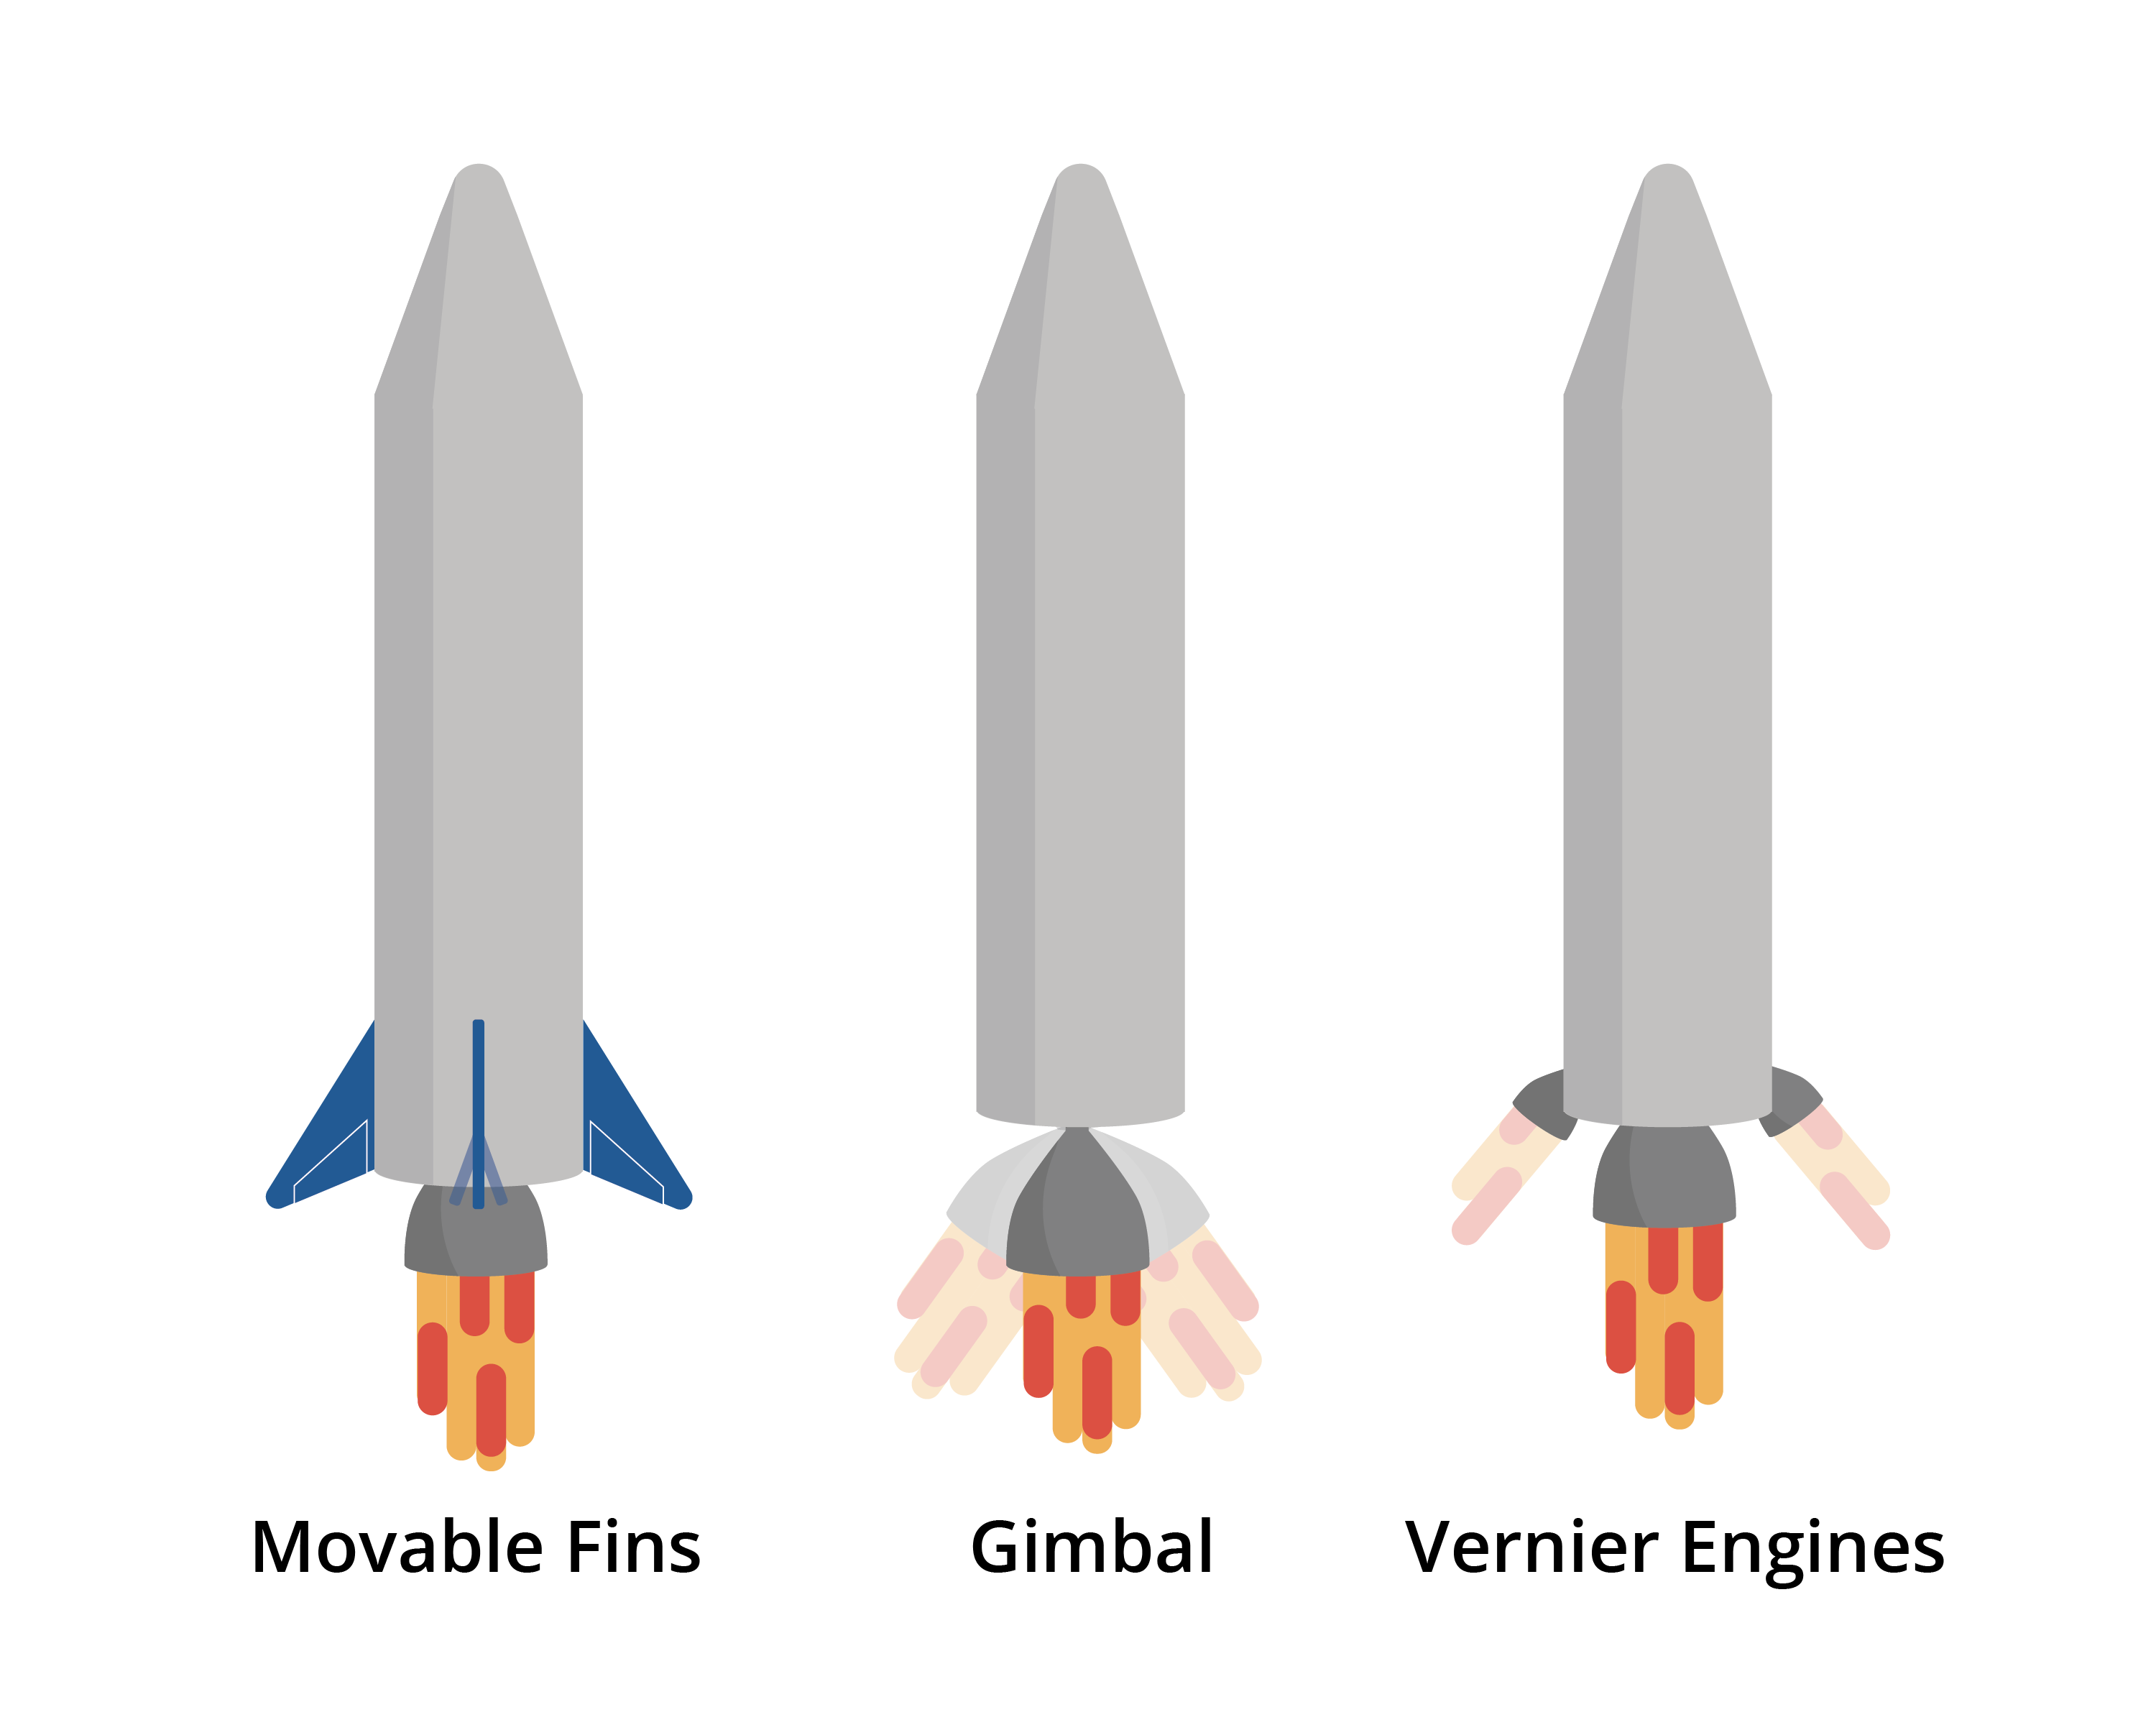
\includegraphics[width=0.75\textwidth]{control.png}
    \caption{Three different methods of engines and their movement in outer space.}
    \label{fig:atmoscontrol}
\end{figure}


\section{Control in space}
\index{rockets ! in space}
The previous section describes ways that engineers control rockets in the atmosphere, but most rockets will end up in the vacuum of space. There are several common ways to adjust the orientation in space.

	One method is using \newterm{RCS thrusters}. An RCS, or reaction control system, is a series of small thrusters that are used to change the direction and position of a spacecraft.
	RCS thrusters are usually small, and placed in blocks of 3-4 allowing for precise control in all three axes. They are often used for docking maneuvers, attitude control, and orbital adjustments. 

	Another method called \newterm{reaction wheels} uses angular momentum to rotate the spacecraft. By accelerating and decelerating wheels on three axes, the spacecraft can rotate in any direction.

	A third common attitude control technology is \newterm{magnetorquer}. Magnetorquers use electromagnets and the earth's magnetic field to adjust the orientation of the spacecraft. Magnetorquers
	are common in small satellites, but they are not as common in larger spacecraft. To manipulate large spacecraft with magnetorquers effectively, you need either prohibitively high current or an external magnetic field
	more powerful than the Earth's magnetic field.

	\subsection*{Pros and Cons of Rocket Control Systems in Space}

	\begin{itemize}
		\item \textbf{RCS Thrusters}
		\begin{itemize}
			\item \textbf{Pros:} Precise control, enables translation and rotation, reliable, effective for docking and attitude adjustments.
			\item \textbf{Cons:} Consumes propellant, limited by onboard fuel, adds weight and complexity.
		\end{itemize}
		\item \textbf{Reaction Wheels}
		\begin{itemize}
			\item \textbf{Pros:} No propellant required, precise attitude control, long operational life, quiet operation.
			\item \textbf{Cons:} Limited torque, can saturate and require desaturation (often using RCS), mechanical failure risk.
		\end{itemize}
		\item \textbf{Magnetorquers}
		\begin{itemize}
			\item \textbf{Pros:} No propellant required, lightweight, simple design, effective for small satellites in low Earth orbit.
			\item \textbf{Cons:} Only works near planetary magnetic fields, limited control authority, not suitable for deep space or large spacecraft.
		\end{itemize}
	\end{itemize}
	
	\begin{figure}[htbp]
		\centering
		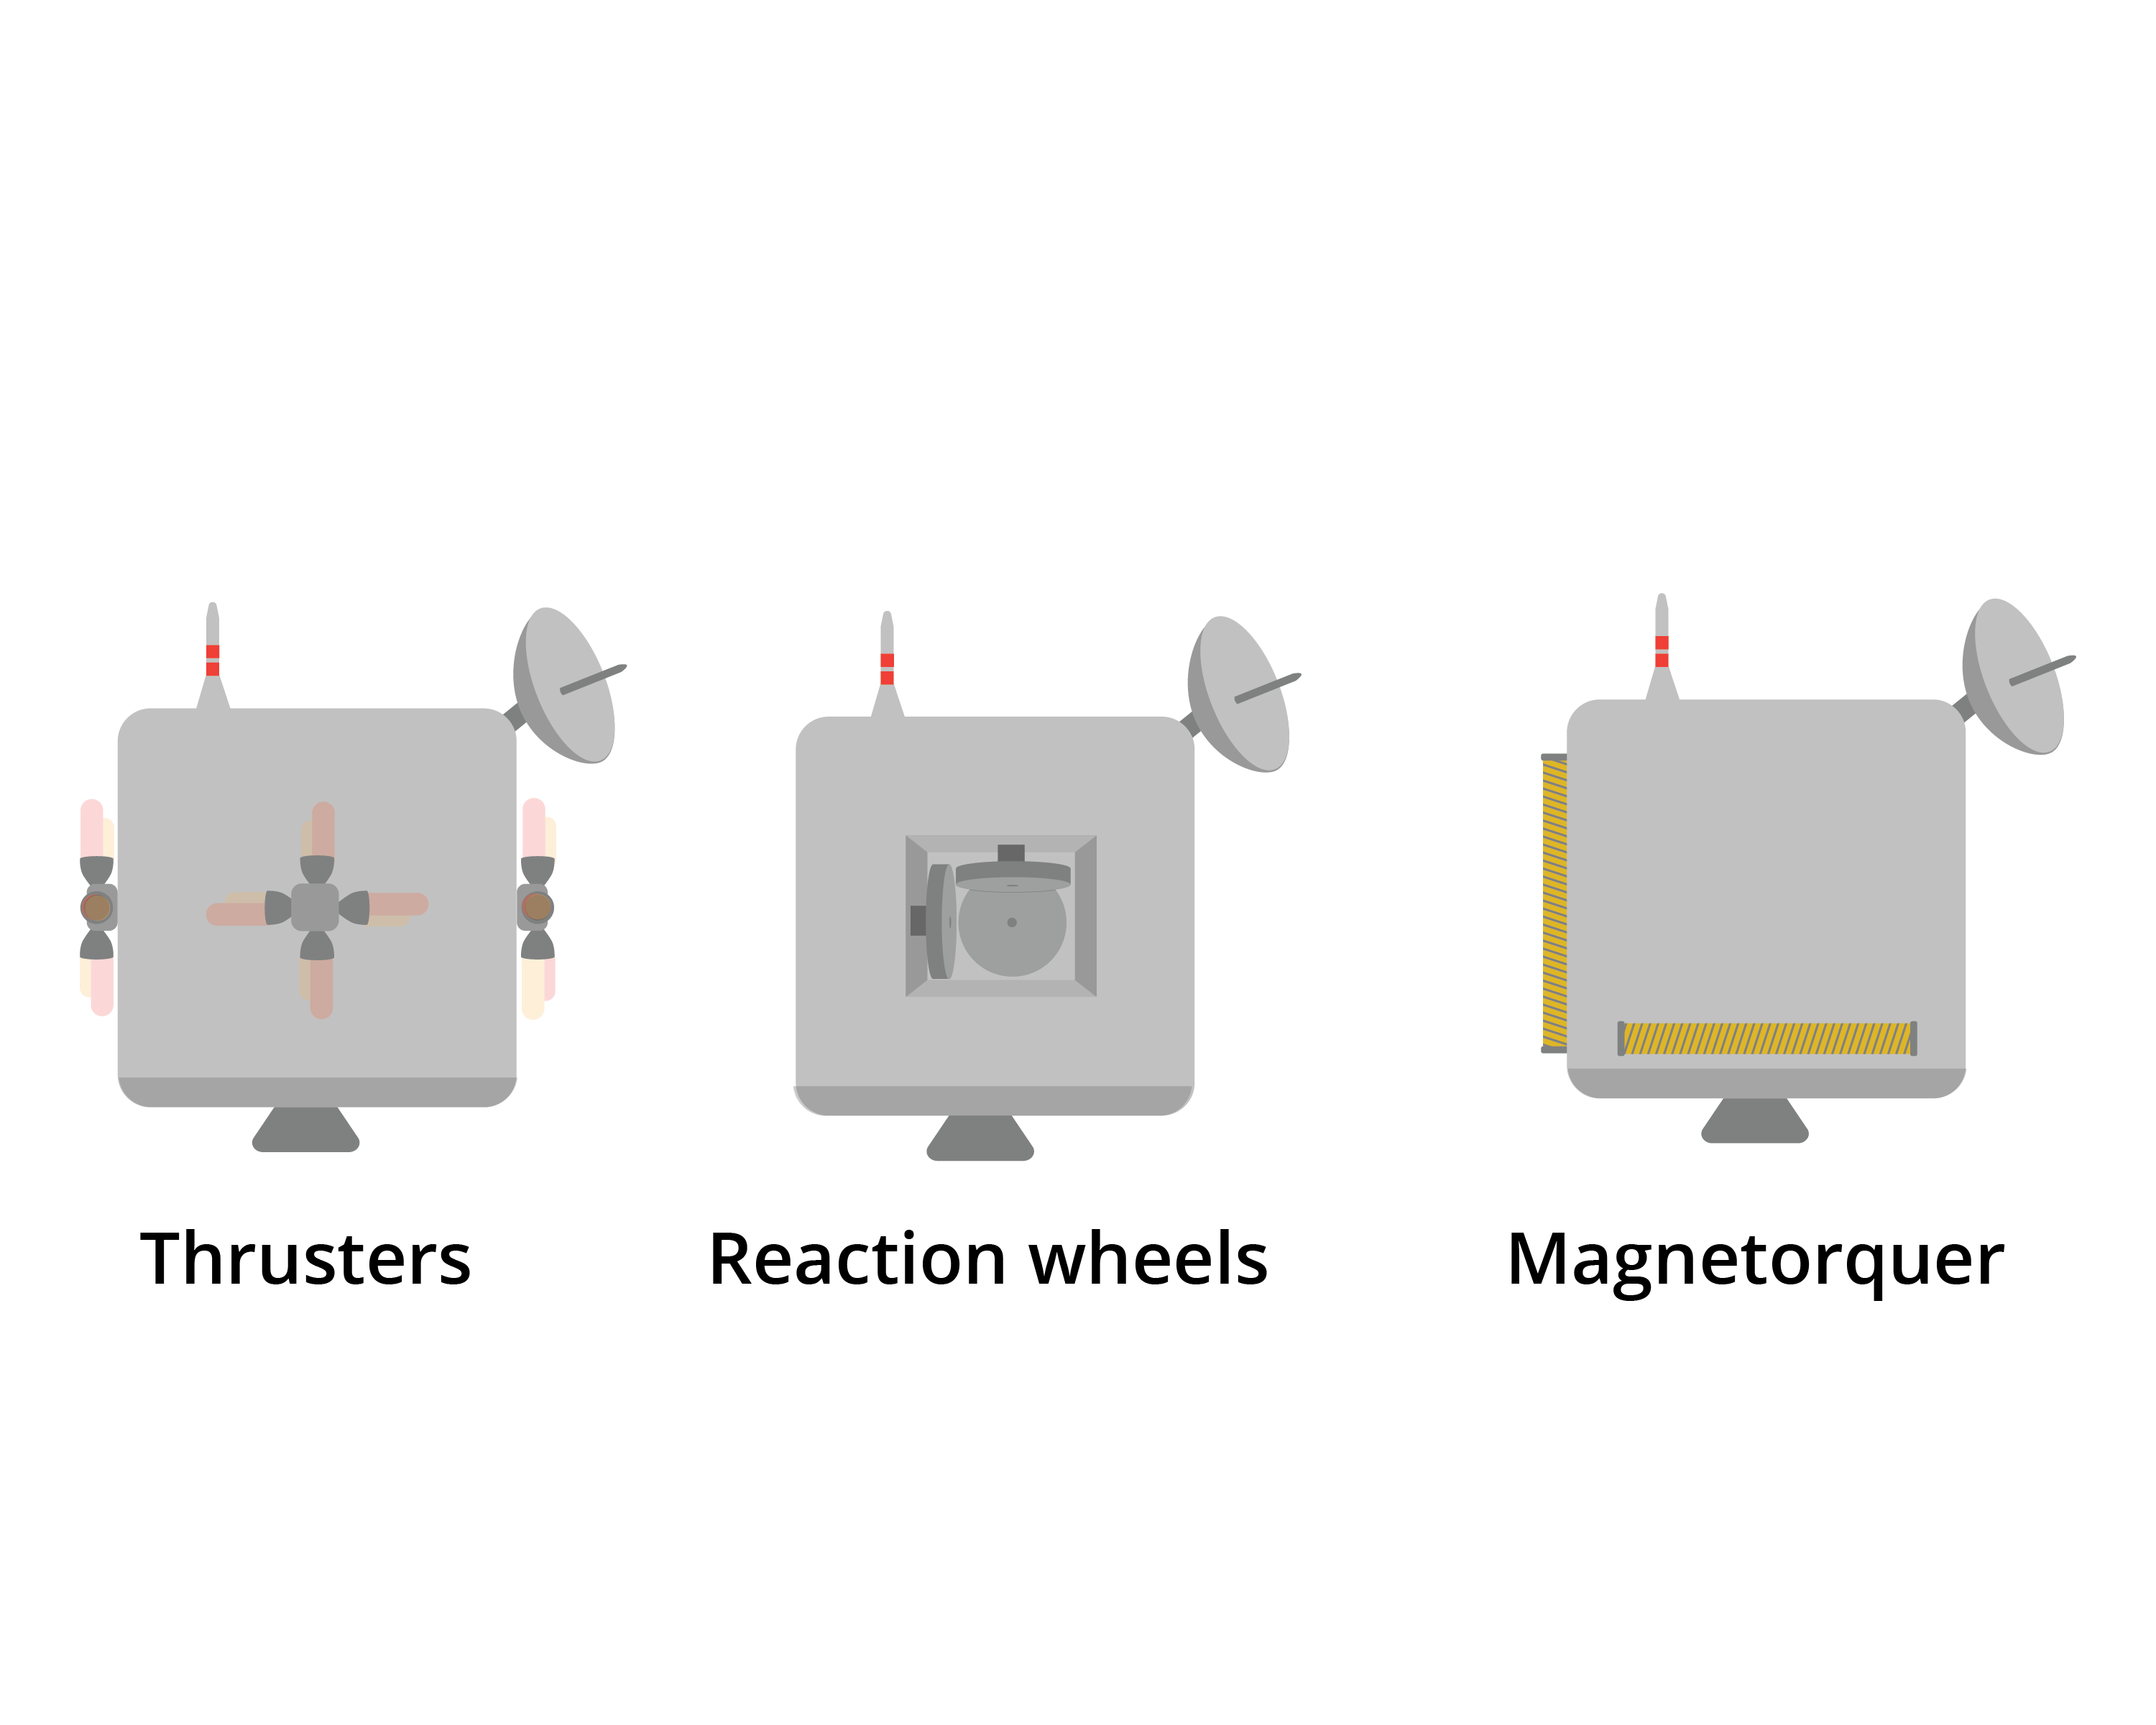
\includegraphics[width=0.75\textwidth]{controlSpace.png}
		\caption{Control options for rockets in space.}
		\label{fig:atmosspace}
	\end{figure}
	


\section{Alternative propulsion}
\index{rockets ! alternate propulsion methods of}

One type of alternate propulsion is called a \newterm{solar sail}. Solar sails use lightweight reflective surfaces to use photons in space to propel the spacecraft without on-board fuel.

\begin{figure}[htbp]
    \centering
	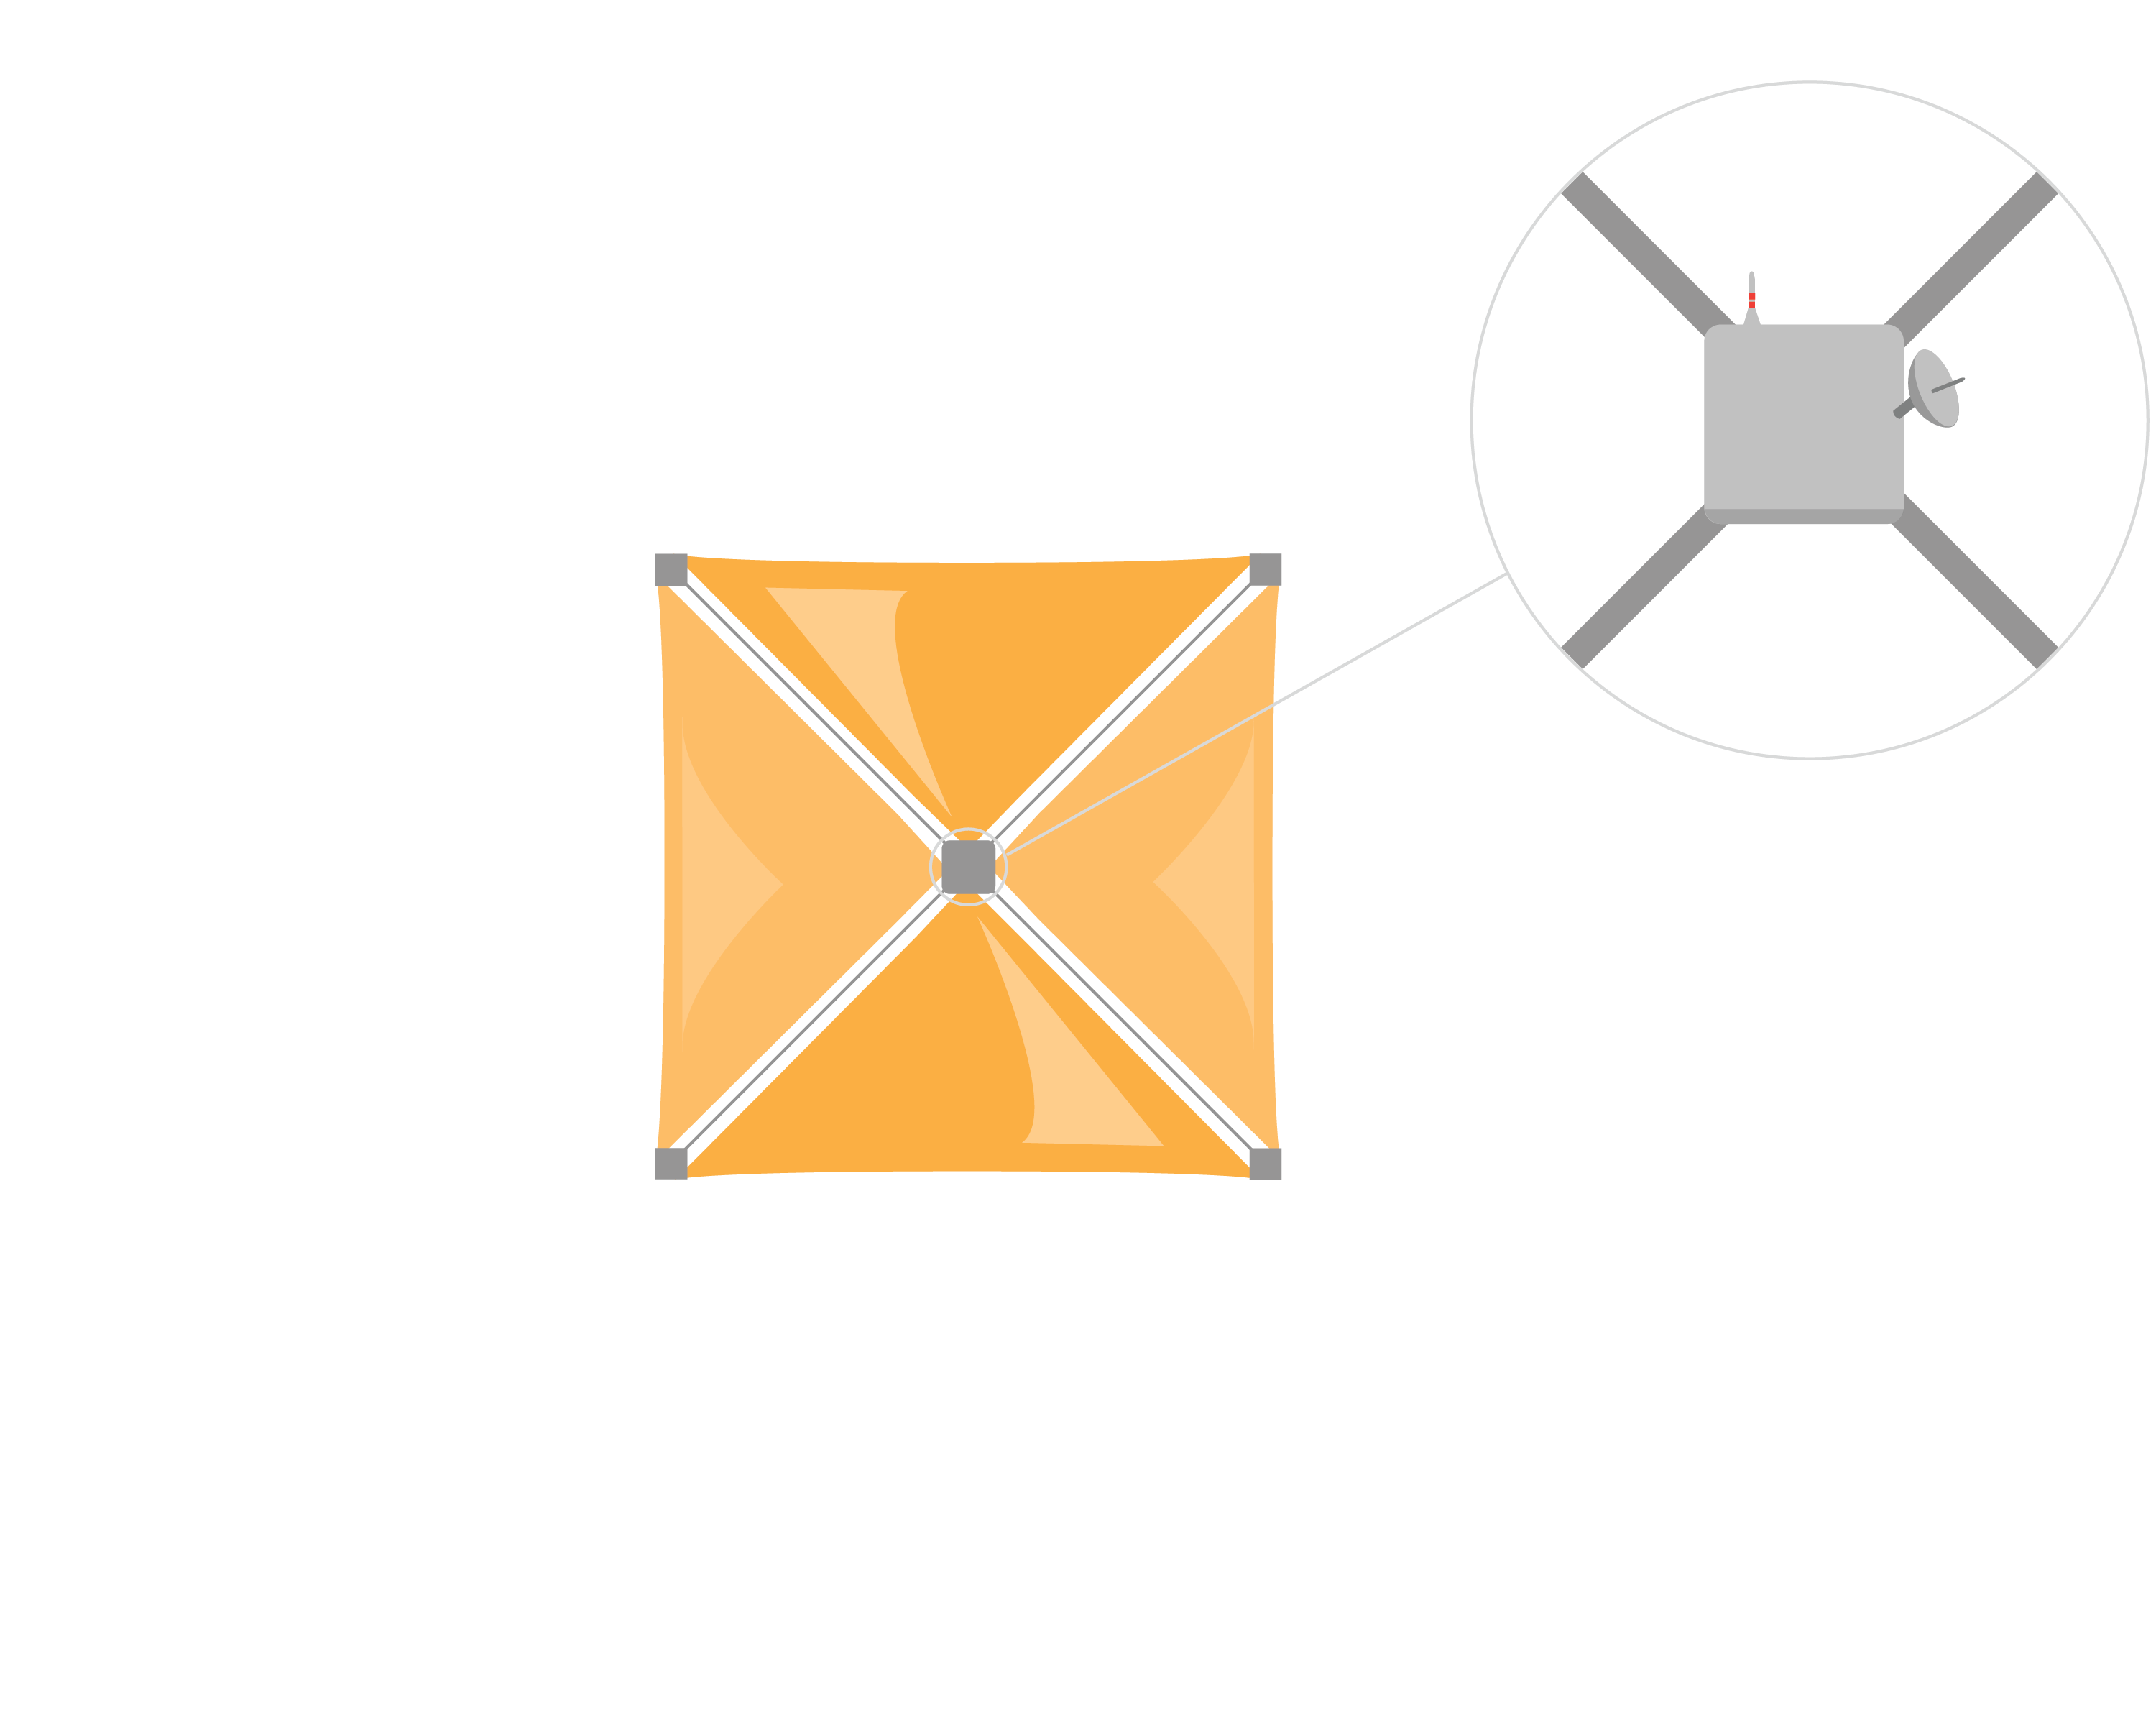
\includegraphics[width=0.75\textwidth]{solarSail.png}
    \caption{Solar sails propel the rocket with photon reflection.}
    \label{fig:solarSail}
\end{figure}

\begin{figure}[htbp]
    \centering
	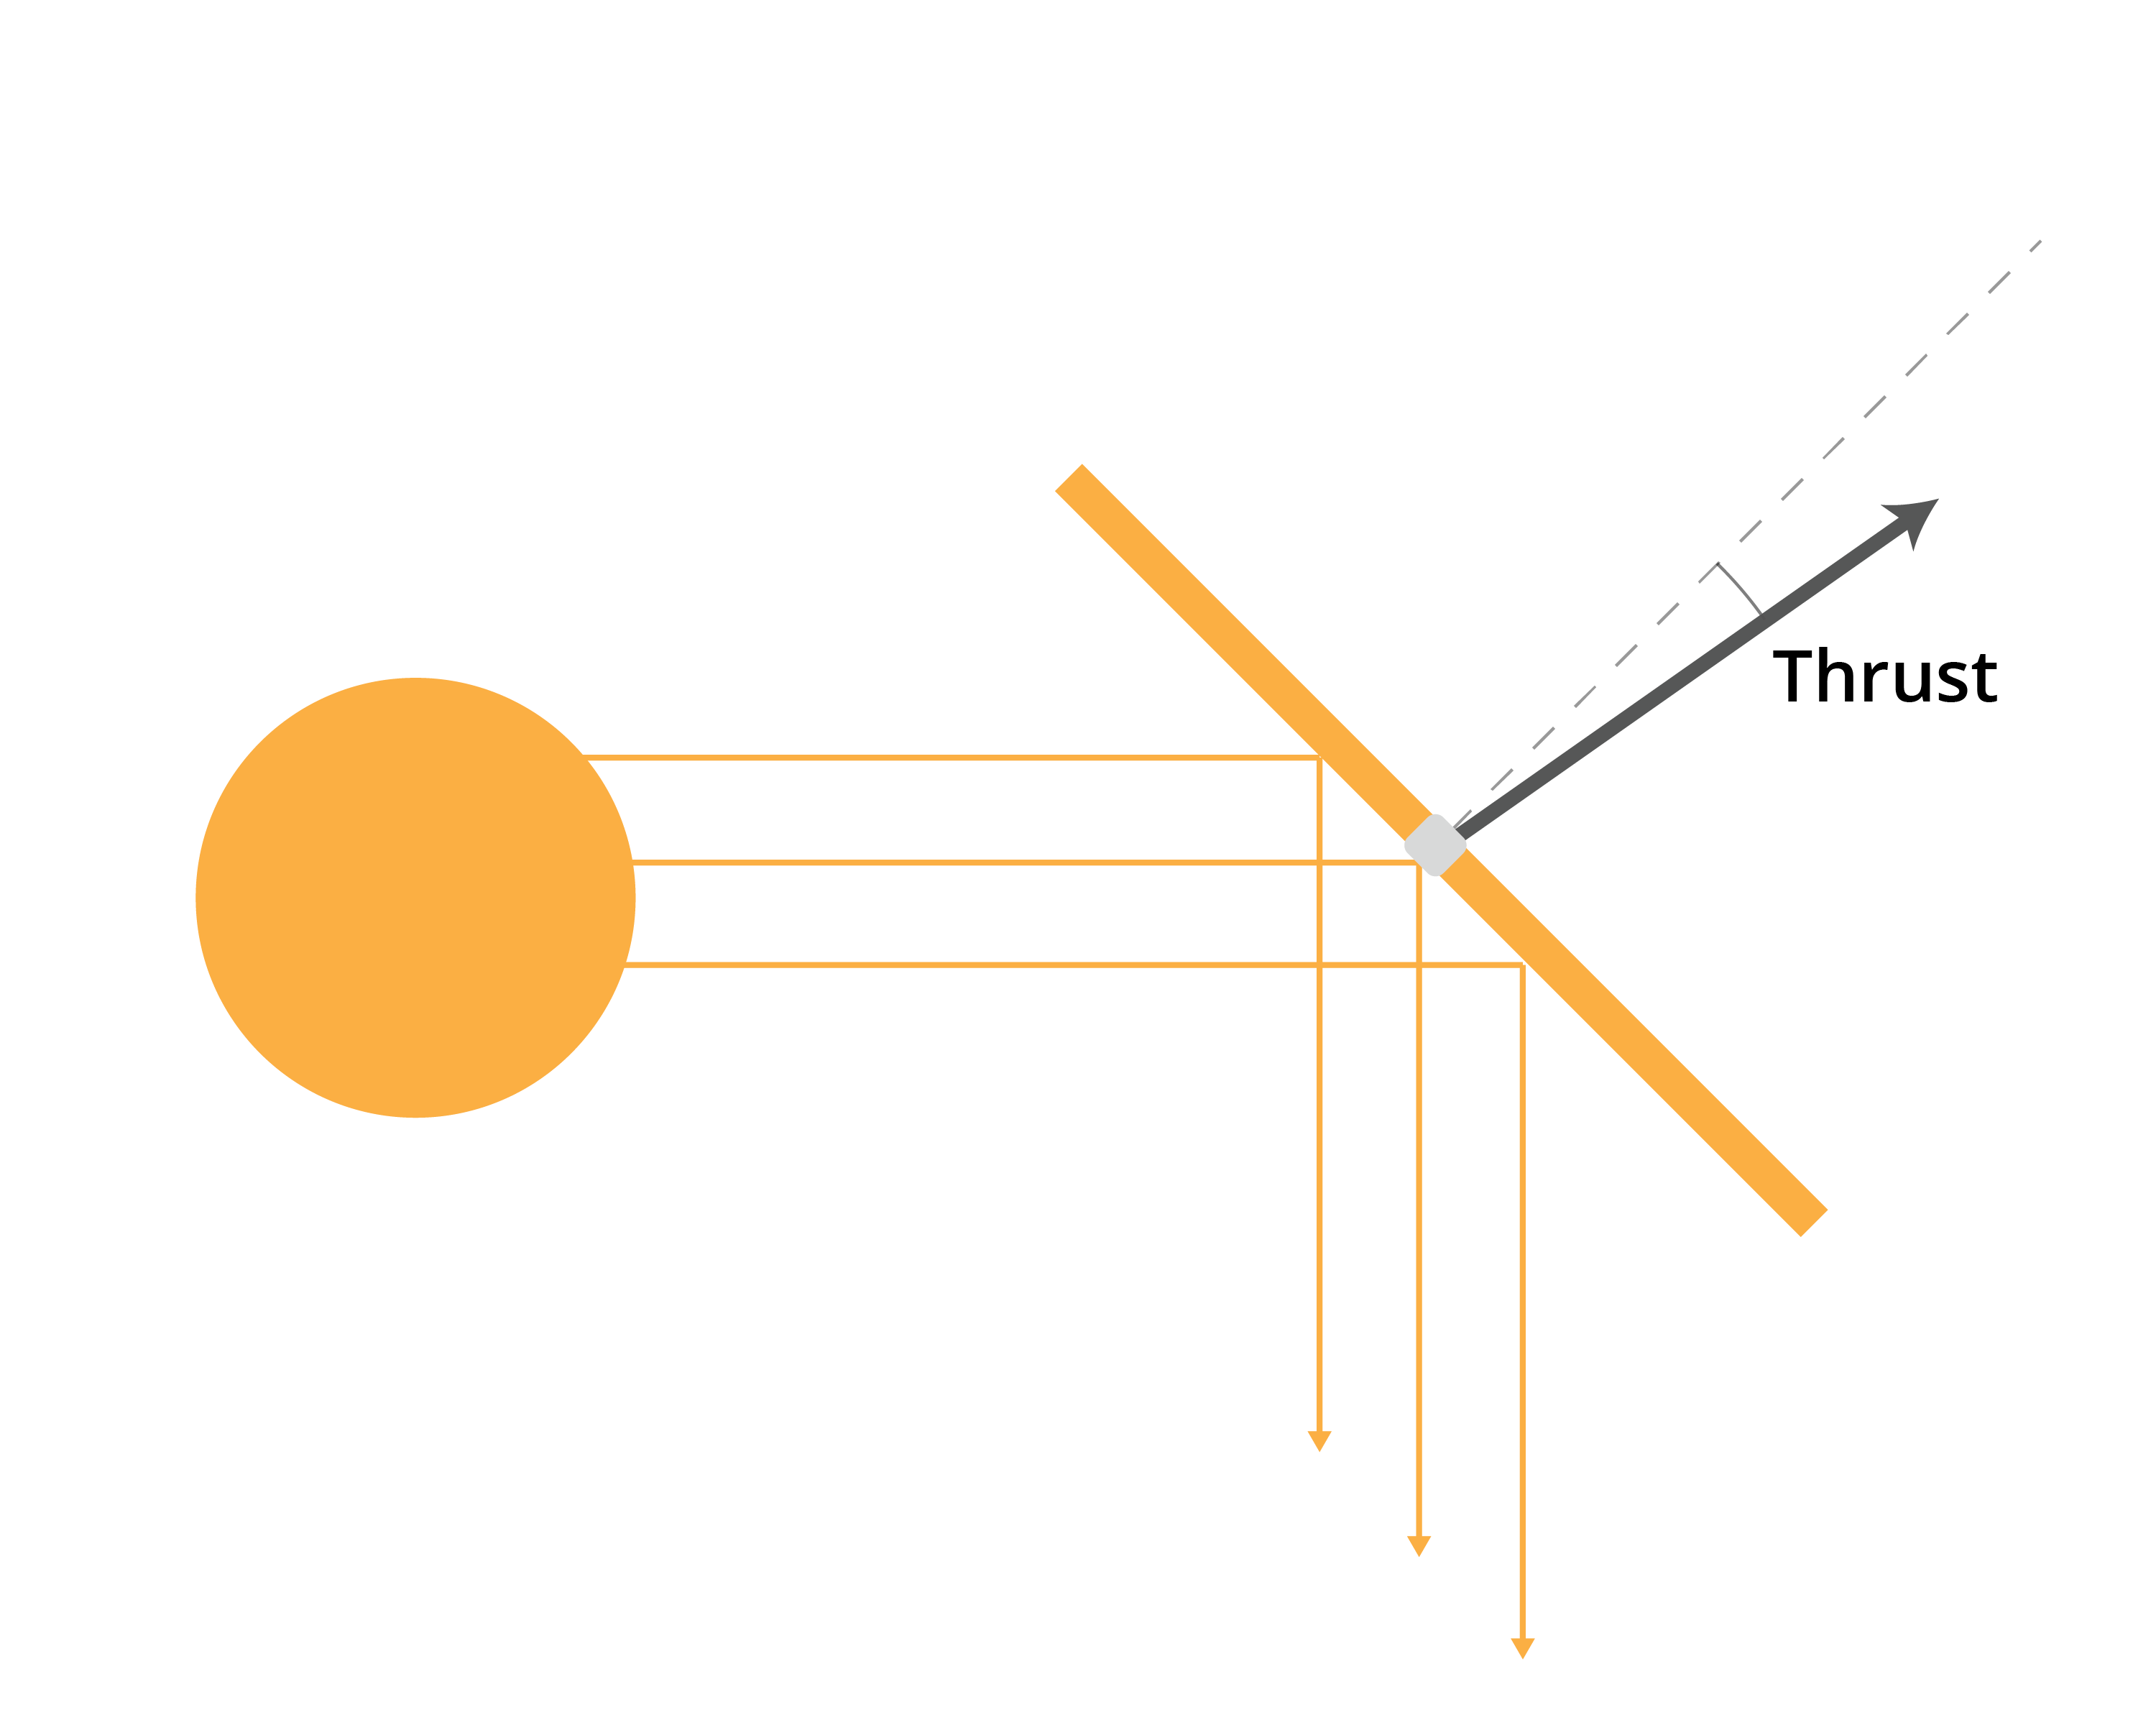
\includegraphics[width=0.75\textwidth]{solarSailDiagram.png}
    \caption{A zoomed in version of solar sails.}
    \label{fig:solarSail}
\end{figure}

Photons reflect off of the surface of the sail. However, since the surface is not perfectly reflective, some of those photons are absorbed, and they produce a horizontal equal and opposite reaction. That small force causes the net thrust to be slightly skewed away from a right angle to the sail.

\newterm{Ion propulsion} is a form of electric propulsion that accelerates ions to generate thrust. There are two main types: electrostatic and electromagnetic. 
Electrostatic ion propulsion uses electric fields to accelerate ions, typically xenon, through grids to produce thrust.  Electrostatic thrusters use the Coulomb 
force to accelerate ions, whereas electromagnetic ion propulsion uses both electric and magnetic fields through the Lorentz force to accelerate ions. Both methods 
are highly efficient and suitable for long-duration space missions, but they produce low thrust compared to chemical rockets.


\begin{figure}[htbp]
    \centering
	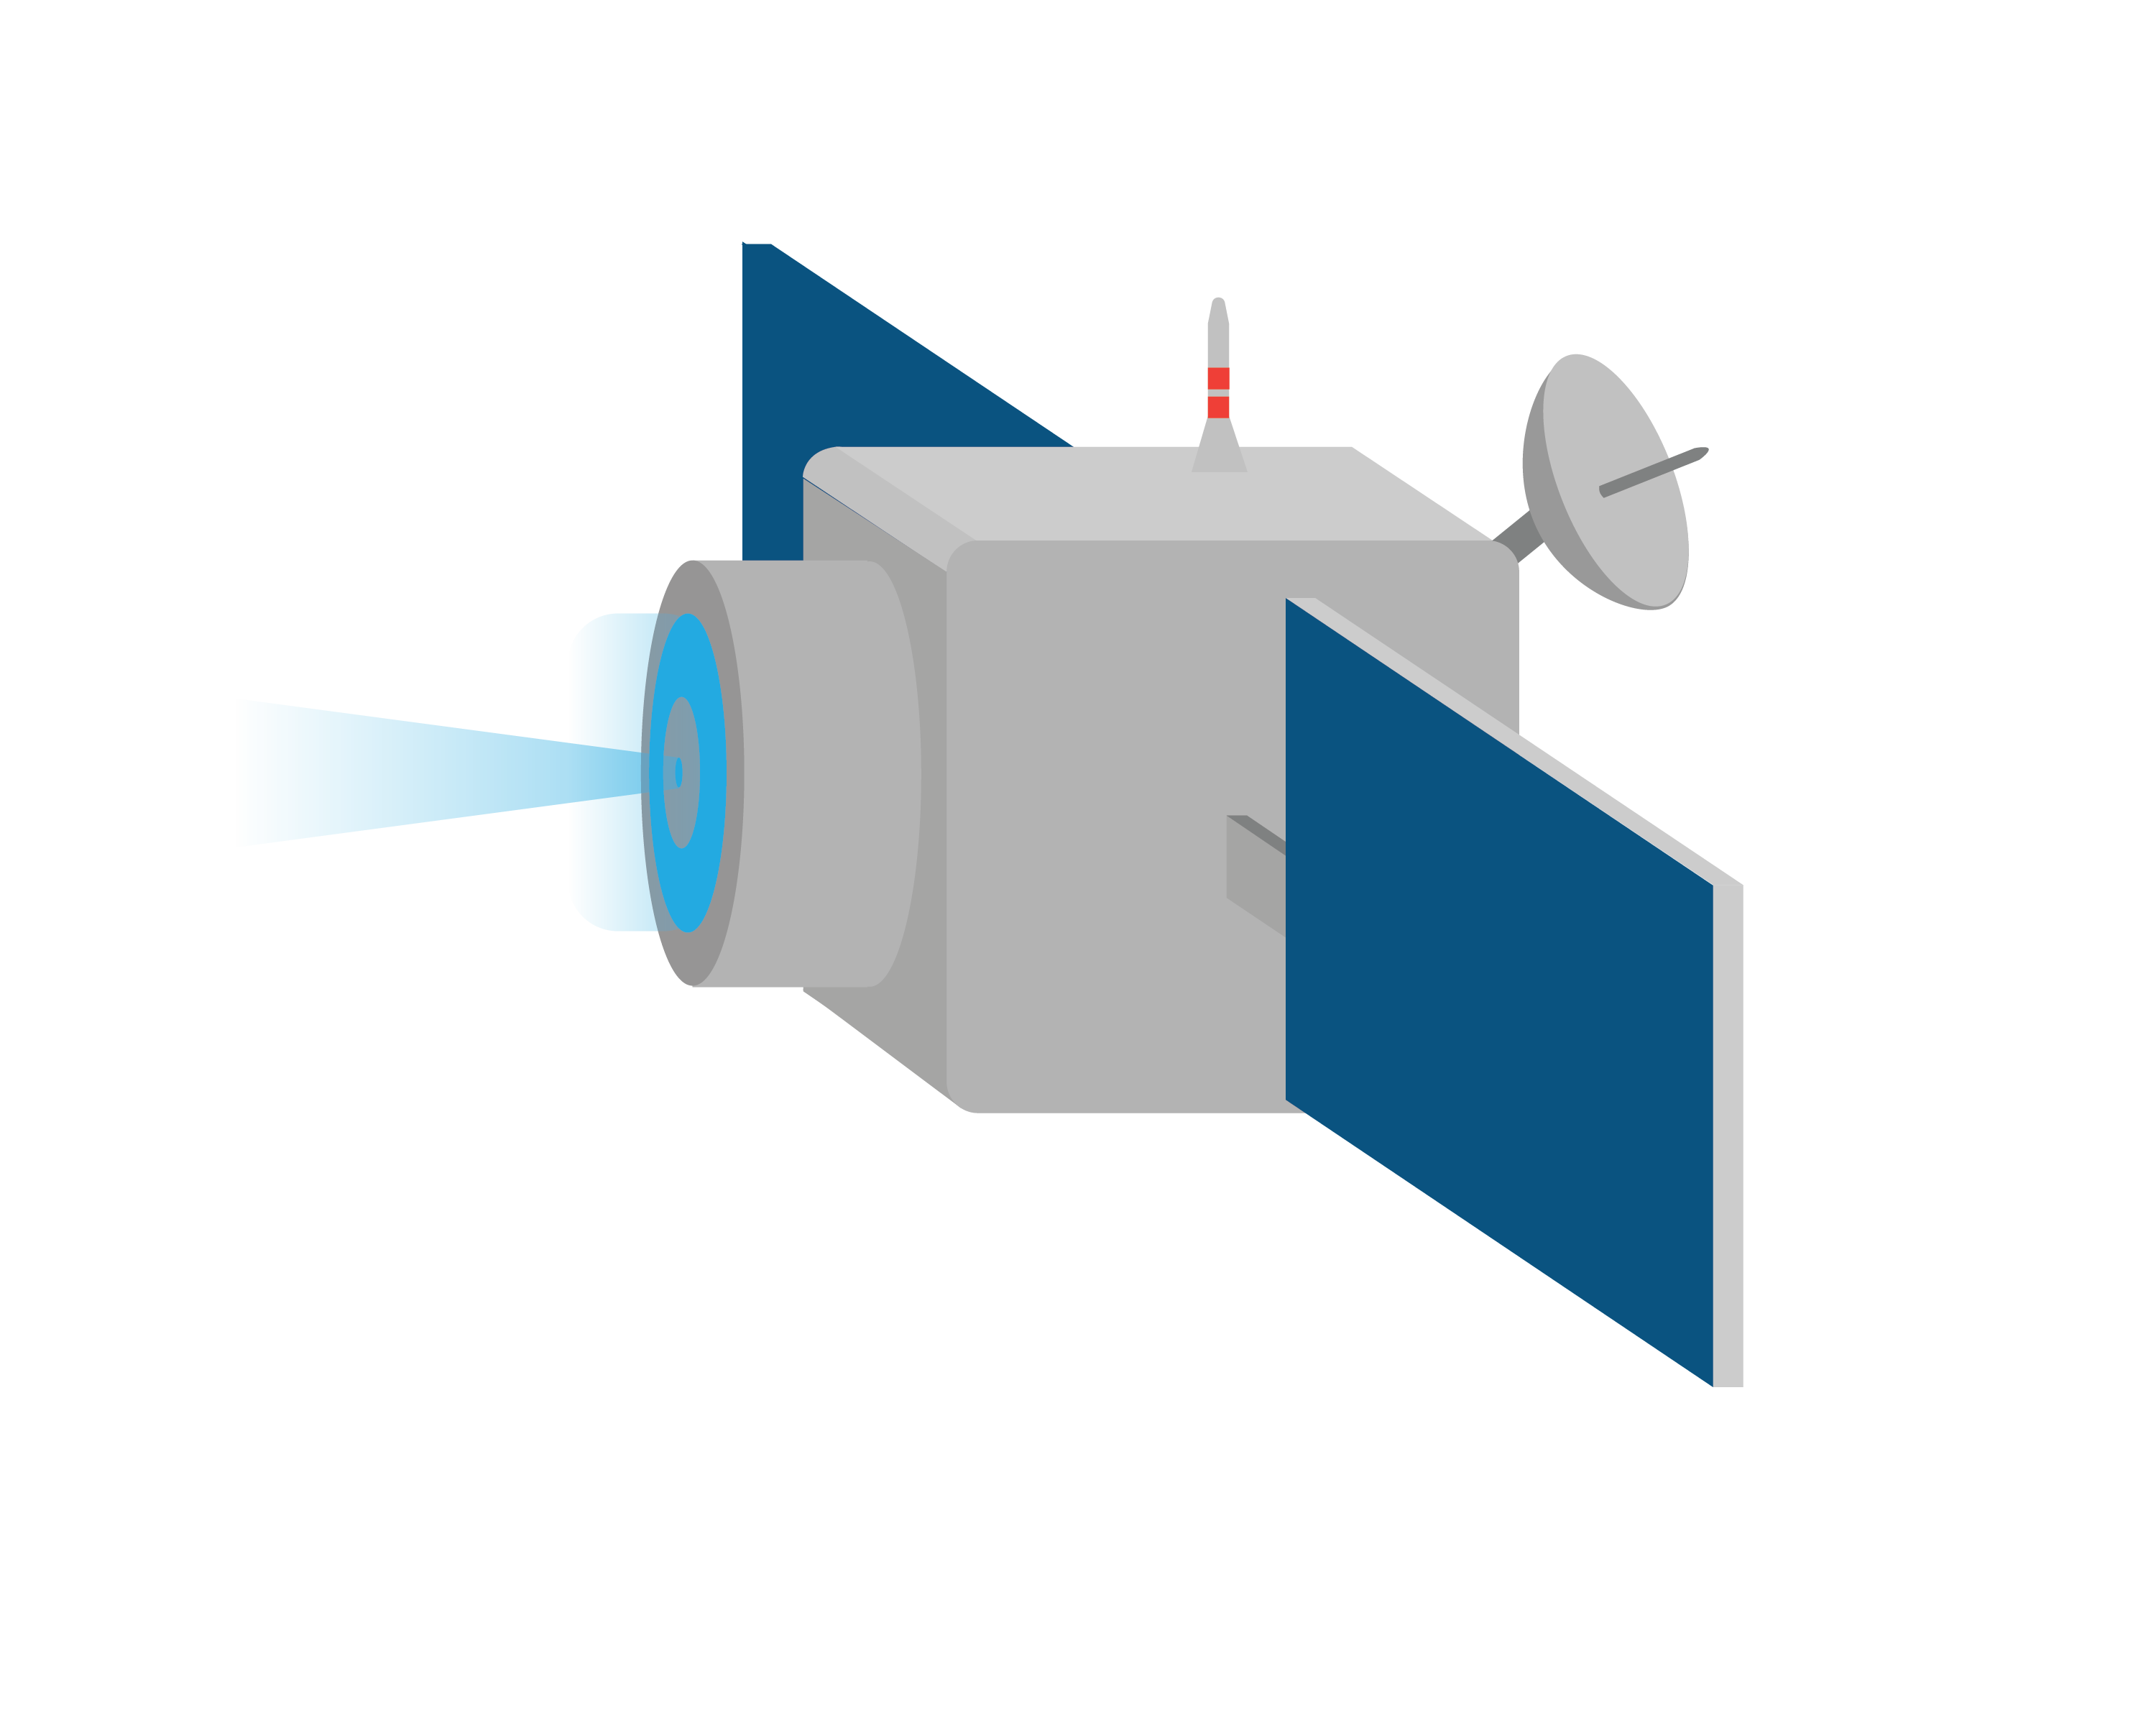
\includegraphics[width=0.75\textwidth]{ionThruster.png}
    \caption{An ion thruster}
    \label{fig:ionThruster}
\end{figure}





